\documentclass[10pt, a4paper]{article}

\usepackage[utf8]{inputenc}
\usepackage[spanish]{babel}
\usepackage{graphicx}
\usepackage{multicol}
\usepackage[usenames,dvipsnames]{color}
\usepackage{amsmath}
\usepackage{verbatim}
\usepackage{footnote}
\usepackage{float}
\usepackage{amsfonts}
\usepackage{hyperref}
\usepackage{framed}
\usepackage{pdflscape}

\usepackage{pdfpages}

\usepackage{caratula}

\newcommand{\NonStandardConector}[2] {
	\item \textbf{#1} : #2
}

\materia{Ingeniería de Software II}

\titulo{Trabajo Práctico 2}
\subtitulo{Developing \textsf{in-the-large} - Planificación}
\grupo{Grupo 5 - \emph{El nene está bien}}

\integrante{Martín Alejandro Miguel}{181/09}{m2.march@gmail.com}
\integrante{Iván Postolski}{216/09}{ivan.postolski@gmail.com}
\integrante{Juan Manuel Martinez Caamaño}{276/09}{jmartinezcaamao@gmail.com}
\integrante{Matías Incem}{396/09}{matias.incem@gmail.com}
\integrante{Pablo Gauna}{334/09}{gaunapablo@gmail.com}

\setcounter{tocdepth}{2}

\begin{document}

\maketitle
\tableofcontents
\newpage

\section{Introducción}

\section{Atributos de calidad}
	\begin{itemize}
\item
  \emph{Extensibilidad} de las fuentes de datos. (2do párrafo enunciado)

  \begin{itemize}
  \item
    Fuente: El equipo de desarrolladores.
  \item
    Estimulo: Se desea implementar una nueva fuente de datos.
  \item
    Artefacto: Sistema de obtención de datos.
  \item
    Entorno: En funcionamiento normal.
  \item
    Respuesta: Se implementa la fuente de datos y se la integra al
    sistema.
  \item
    Medida: La fuente de datos se integra con el sistema en menos de 1
    hora, sin detener al sistema.
  \end{itemize}
\item
  \emph{Modificabilidad} de los bots que obtienen datos.

  \begin{itemize}
  \item
    Fuente: El equipo de desarrolladores.
  \item
    Estimulo: Se desea implementar/modificar/eliminar un bot para
    obtener datos de una pagina web determinada.
  \item
    Artefacto: Sistema de obtención de datos.
  \item
    Entorno: En funcionamiento normal.
  \item
    Respuesta: Se implementa el bot y se integra con el sistema.
  \item
    Medida: el bot se implementa o modifica en menos de 25 horas y se
    integra con el sistema en menos de 1 hora, sin detener al sistema.
  \end{itemize}
\item
  \emph{Detección de fallas} en la información obtenida por los bots.

  \begin{itemize}
  \item
    Fuente: Las paginas monitoreadas.
  \item
    Estimulo: Se produce un cambio en la estructura de las paginas
    monitoreadas.
  \item
    Artefacto: Bot del sistema de obtención de datos.
  \item
    Entorno: En funcionamiento normal.
  \item
    Respuesta: Se detecta el cambio en la estructura de la pagina, se
    detiene el bot, y se informa a los administradores.
  \item
    Medida: Cuando de una serie de consultas, se detecta un 70\% de
    cambios en su estructura, se considera como error.
  \end{itemize}
\item
  \emph{Modificabilidad} de los rubros y productos de rubros. (3pe)

  \begin{itemize}
  \item
    Fuente: Administradores del sistema.
  \item
    Estimulo: Se desea agregar un nuevo producto/rubro.
  \item
    Artefacto: Sistema central TPA.
  \item
    Entorno: Funcionamiento normal.
  \item
    Respuesta: Utilizando la interfaz de administración, se agrega un
    nuevo producto/rubro al sistema, sin detenerlo.
  \item
    Medida: Se agrega un producto/rubro en menos de 5 minutos.
  \end{itemize}
\item
  \emph{Modificabilidad} de las reglas de asociación y sustitución.
  (3pe)

  \begin{itemize}
  \item
    Fuente: Administradores del sistema
  \item
    Estimulo: Se desea agregar/modificar las reglas de asociación y
    sustitución.
  \item
    Artefacto: Sistema central TPA.
  \item
    Entorno: Modo de mantenimiento.
  \item
    Respuesta: Se modifican las reglas de asociación y sustitución.
  \item
    Medida: En menos de 24hs se implementan y ponen en funcionamiento
    las modificaciones a estas reglas.
  \end{itemize}
\item
  \emph{Performance} para velocidad en que se identifican ofertas de las
  distintas fuentes de datos. (4pe)

  \begin{itemize}
  \item
    Fuente: Usuario externo
  \item
    Estimulo: Se publica en un medio monitoreado por el sistema de
    obtención de datos una oferta.
  \item
    Artefacto: Sistema de obtención de datos.
  \item
    Entorno: Funcionamiento normal.
  \item
    Respuesta: El sistema de obtención de datos identifica esta oferta y
    la agrega a la base de datos.
  \item
    Medida: La oferta se comienza a tener en cuenta 10 segundos despues
    de que fue publicada por una fuente de datos.
  \end{itemize}
\item
  \emph{Usabilidad}, sistema de confianza facilmente configurable.

  \begin{itemize}
  \item
    Fuente: Usuario autentificado.
  \item
    Estimulo: Modifica las reglas de confianza de ofertas.
  \item
    Artefacto: Sistema central TPA.
  \item
    Entorno: Funcionamiento normal.
  \item
    Respuesta: Se modifican las reglas de confianza de ofertas.
  \item
    Medida: El sistema provee una guia de configuración de confianza de
    ofertas, que ayuda a completar dicha tarea en menos de 15 minutos
    para un usuario nuevo.
  \end{itemize}
\item
  \emph{Extensibilidad} de las fuentes de confianza de datos del
  usuario.

  \begin{itemize}
  \item
    Fuente: Equipo de desarrollo.
  \item
    Estimulo: Se desea agregar una nueva fuente de confianza de datos
    del usuario.
  \item
    Artefacto: Sistema central TPA.
  \item
    Entorno: Modo de mantenimiento.
  \item
    Respuesta: Se agrega la fuente de confianza de datos al sistema.
  \item
    Medida: La fuente de confianza se implementa en menos de 25hs y se
    integra al sistema en menos de 1 hora.
  \end{itemize}
\item
  \emph{Modificabilidad} del servicio de deteccion de spam.

  \begin{itemize}
  \item
    Fuente: Equipo de desarrollo.
  \item
    Estimulo: Se desea modificar el funcionamiento del servicio de
    detección de Spam.
  \item
    Artefacto: Sistema de detección de Spam.
  \item
    Entorno: Funcionamiento normal.
  \item
    Respuesta: Se modifica el funcionamiento del servicio.
  \item
    Medida: El funcionamiento del servicio de detección de Spam debe
    poder modificarse (Cambio de proveedor, nuevo proveedor,
    etc\ldots{}) con el sistema en funcionamiento Normal, y deberia ser
    posible que mas de un sistema de detección de Spam puedan
    co-existir.
  \end{itemize}
\item
  \emph{Auditabilidad} para ver la cantidad de ofertas falsas
  detectadas, productos de precios dudosos, etc.

  \begin{itemize}
  \item
    Fuente: Administradores del sistema.
  \item
    Estimulo: Se desea ver el resumen de ofertas falsas, detectadas,
    etc\ldots{}
  \item
    Artefacto: Sistema de detección de Spam.
  \item
    Entorno: Funcionamiento normal.
  \item
    Respuesta: Se obtiene un resumen con la información de ofertas
    falsas detectadas, precios dudosos, etc\ldots{}
  \item
    Medida: Cada vez que se elimina / modifica una oferta se registra
    `quien, cuando, por que (precio dudoso, oferta falsa, etc\ldots{}),
    y la oferta'.
  \end{itemize}
\item
  \emph{Usabilidad} de la interfaz del sistema para realizar consultas.

  \begin{itemize}
  \item
    Fuente: Un usuario nuevo.
  \item
    Estimulo: El usuario desea realizar una consulta.
  \item
    Artefacto: Interfaz Movil / Interfaz Web.
  \item
    Entorno: Funcionamiento normal.
  \item
    Respuesta: Se realiza la consulta y se informa de los resultados a
    los usuarios.
  \item
    Medida: En menos de 5 minutos, un usuario nuevo comprende la
    interfaz y comienza a utilizarla .
  \end{itemize}
\item
  \emph{Usabilidad} de la interfaz del sistema mientras se realizan
  consultas.

  \begin{itemize}
  \item
    Fuente: Un usuario.
  \item
    Estimulo: El usuario desea realizar una consulta.
  \item
    Artefacto: Interfaz Movil / Interfaz Web.
  \item
    Entorno: Funcionamiento normal.
  \item
    Respuesta: Conforme se escribe la respuesta, se muestran resultados.
  \item
    Medida: En menos de 1 segundo luego de que se comenzo a tipear una
    consulta, el sistema comienza a sugerir posibles resultados.
  \end{itemize}
\item
  \emph{Usabilidad} de la interfaz del sistema, antes de realizar
  consultas.

  \begin{itemize}
  \item
    Fuente: Un usuario.
  \item
    Estimulo: Se accede a la interfaz y aun no se realiza ningun tipo de
    consulta.
  \item
    Artefacto: Interfaz Movil / Interfaz Web.
  \item
    Entorno: Funcionamiento normal.
  \item
    Respuesta: Se comienzan a presentar resultados.
  \item
    Medida: Se muestran las ofertas populares / mas buscadas / mas
    recomendadas.
  \end{itemize}
\item
  \emph{Disponibilidad} del servicio.

  \begin{itemize}
  \item
    Fuente: Usuario.
  \item
    Estimulo: Se desea realizar una consulta.
  \item
    Artefacto: Interfaz movil.
  \item
    Entorno: Funcionamiento normal.
  \item
    Respuesta: Se realiza la consulta al sistema, se obtienen resultados
    y son mostrados al usuario.
  \item
    Medida: En el 99\% de los casos la consulta se realiza con exito al
    sistema central.
  \end{itemize}
\item
  \emph{Disponibilidad} del servicio cuando no hay conección.

  \begin{itemize}
  \item
    Fuente: Usuario.
  \item
    Estimulo: Se desea realizar una consulta.
  \item
    Artefacto: Interfaz movil.
  \item
    Entorno: Funcionamiento sin conección
  \item
    Respuesta: Si la consulta se encuentra disponible sin conección, se
    obtienen los resultados y son mostrados al usuario.
  \item
    Medida: Las ultimas consultas y las consultas mas populares al
    momento de la ultima conección se encuentran disponibles.
  \end{itemize}
\end{itemize}


\section{Arquitectura}

\subsection{Referencia de conectores}
A continuación presentamos una referencia a los conectores utilizados en los diagramas que se presentaran en las siguientes secciones. Los conectores \emph{no-standard} utlizados son especificados mas abajo.

\begin{figure}[H]
	\centering
	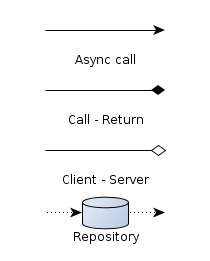
\includegraphics[scale=0.6]{graficos/call_reference.png}
	\caption{Referencia de conectores.}
\end{figure}

\subsubsection{Conectores no estandar}

\begin{itemize}
		%Completar con conectores no standard!
		%Agregar asi:
		\NonStandardConector{A non standard conector name}{A non standard conector description.}
\end{itemize}

\subsection{Subsistema de Query}

En el siguiente diagrama presenta el \textsf{Subsistema de Query} donde dada una consulta por productos (\textbf{query}) se arma la respuesta al usuario que realizó la consulta. En este diagrama se encuentran ejemplificados los \emph{casos de uso} 7, 8, 9, 10, 11 y 12.

\begin{figure}[H]
	\centering
	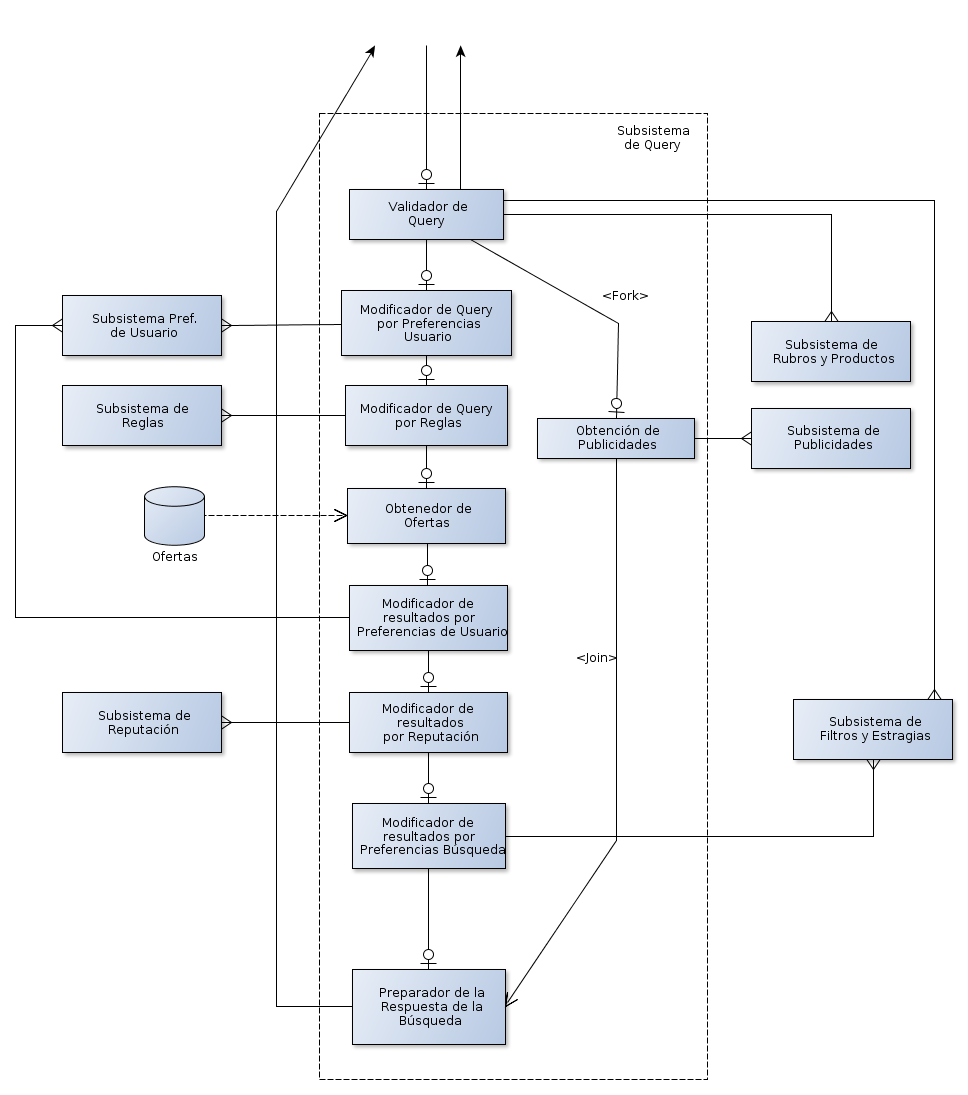
\includegraphics[width=\textwidth]{graficos/arch/subsistema_query.png}
	\caption{Diagrama arquitectónico con el detalle del \textsf{Subsistema de Query}.}
\end{figure}

\subsection{Interfaz movil}

\begin{figure}[H]
	\centering
	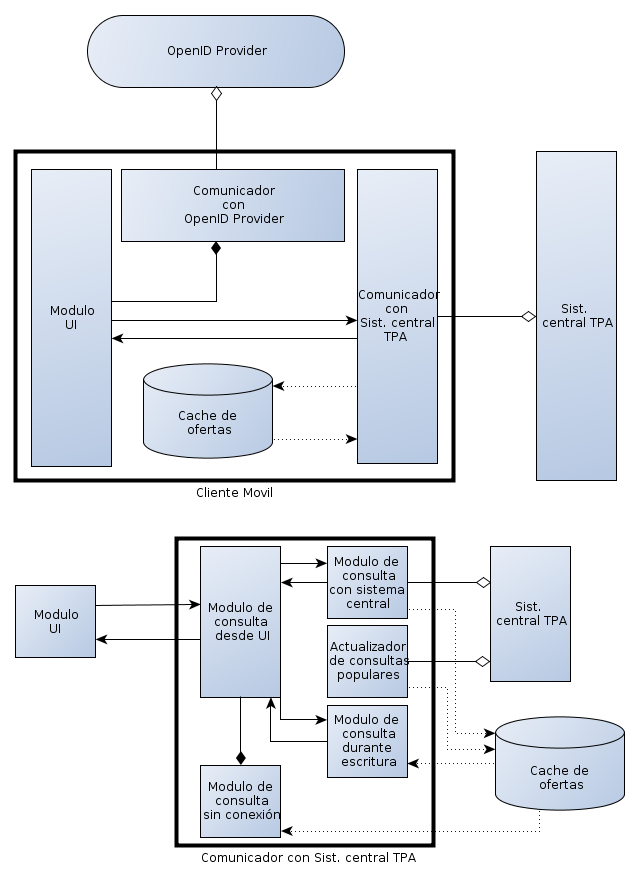
\includegraphics[width=\textwidth]{graficos/arch/Cliente_movil.png}
	\caption{Diagrama arquitectónico con el detalle del \textsf{Cliente movil}.}
\end{figure}



\end{document}
